\documentclass{article}
\usepackage{amsmath}
\usepackage{gensymb}
\usepackage{float}
\usepackage[top=1in, bottom=1in, left=1in, right=1in]{geometry}
\usepackage{graphicx}
\usepackage{rotating}
\usepackage{multirow}
\usepackage{wrapfig}
\usepackage{array}
\usepackage{float}
\usepackage{caption}
\usepackage{subcaption}
\usepackage{ragged2e}
\usepackage[hidelinks]{hyperref}
\makeatletter
\newcommand*{\rom}[1]{\expandafter\@slowromancap\romannumeral #1@}
\makeatother
\graphicspath{ {Data/} }
\begin{document}
	\everymath{\displaystyle}
	\begin{titlepage}	 	
		\center
		\text{}\\[3cm]
		\linespread{2}\Huge \bfseries MP1: Metric Learning
		\center\textsc{\Large ECE 417 Fall 2017}\\[1cm]
		\Large\center\textsc{Weicheng Jiang \\Yuchen Liang\\ Zixu Zhang  }\\[1.5cm]
		\Large \today\\
		\vfill
	\end{titlepage}
	%\tableofcontents\newpage
	\setlength{\baselineskip}{24pt}
	
	\section{Introduction}
	
	In this MP, a database of 1400 images is provided, together with 47 features for each image (i.e. a $47\times1400$ matrix, stored as handles.META\_DATA). The goal of this MP is to find the most relevant (defined by the user) 20 images with respect to the given one, through optimization from repeated user feedback. A list of feature vectors, corresponding to various implicit image features (determined by the feature extracting algorithm), are being used in this experiment, for what matters here is the relationship between pixels rather than each raw pixel itself.
	
	\justify In determining the highest relevance, we use the Mahalanobis distance metric. The algorithm learns the weighting matrix W, a matrix that determines the level of relevance among 47 different features, from user feedback on the training set. The algorithm updated W every round to arrange larger weight for those features that the user is more interested.
	
	
	\section{Methods}
	
	The two critical parts of this experiment are 1) how to output the images with highest relevance given the weight of each feature (i.e. the weighting matrix W) and 2) how to update W to correspond to the highest relevance from user feedback.
	
	\justify On line 164, we compute the Mahalanobis distance between the given image and all the images in the database, with respect to each feature value, using the following equation:
	$$D(j)=(\mathbf{q}_c-\mathbf{x}_j)^T\mathbf{W}(\mathbf{q}_c-\mathbf{x}_j)$$ where $\mathbf{q}_c$ is the mean relevant image feature vector and $\mathbf{x}_j$ is the $j^{th}$ database image feature-vector. A smaller distance indicates a higher relevance, and the most relevant 20 images are output in the next round.
	
	\justify Starting line 225, we update $\mathbf{W}$ after each round of user feedback except the first round where we set $\mathbf{W}$ to be an identity matrix, using the following equation:
	$$W(i,i)=\frac{1}{\sigma^2_i+0.0222}$$
	where $\sigma_i^2$ is the variance of each feature vector among the positive (relevant) images in the feedback, and 0.0222 is added for regularization. If some features among the positive (relevant) images are lower in variance, they are more likely to be the features that the user wants, and higher weights will be allocated to those features.
	
	\section{Results}
	We experimented the learning algorithm on five random images, each with three trials (where a trial is defined to be one feedback round). The first trial outputs images randomly, while the later two trials make use of the distance metric. The rate of precision (defined to be the percentage of relevant images determined by the user) is computed in every trial. Figure \ref{fig: 1} shows the percision changes with number of trails on five different images. A five rounds test is also conducted, and its results are shown in Figure \ref{fig: 2}.
	\begin{figure}[H]
		\centering
		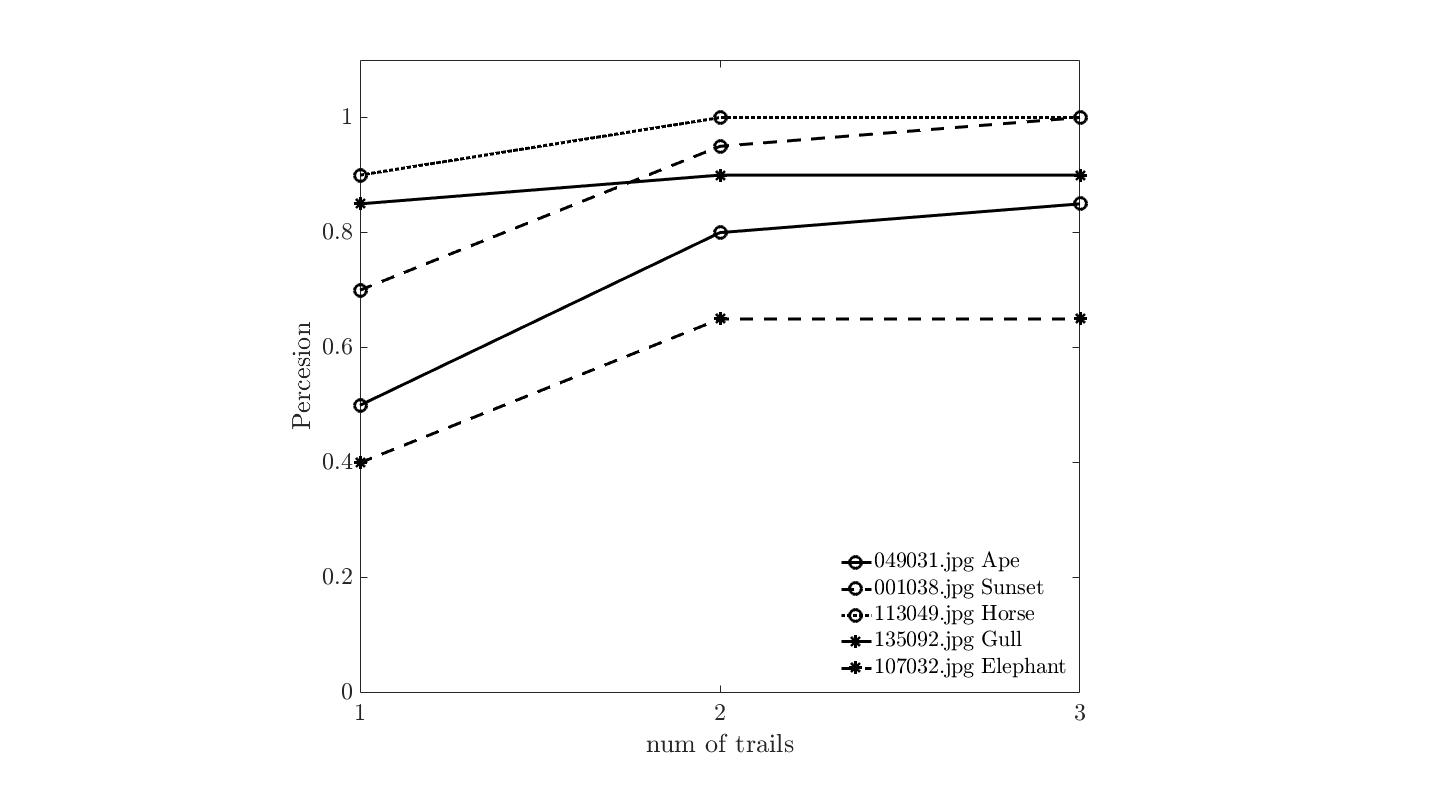
\includegraphics[width=\linewidth]{fig_1}
		\caption{Percision with three rounds of query}
		\label{fig: 1}
	\end{figure}

	
	
	\section{Discussion}
	
	Take the rate of precision of Ape (049031.jpg) as an example. The precision starts at 0.5, which is based on pure guess. At the second trial, the precision jumps to 0.8, because the algorithm puts higher weights on some of the features, recognized by human as the features of apes, and then outputs those images in the database with the closest distances to the mean feature values. In the third trial, the precision rate increases to an even higher value, 0.85.
	
	\justify The difference in the growth of precision rate among the images can be due to i) the features recognized by the program, and ii) the weighting matrix. Since the provided features are those recognized by the program rather than human beings, what a human thinks to be a feature of a particular object may not lie within any collection of features provided by the program. Besides, the weighting matrix are diagonal, implicitly ignoring the underlying covariance among different features. Hence, results from some of the images can grow at a much lower pace than those from others. Therefore, precision vs. number of rounds for some of the test images may change at different rates. 
	
	
	\section{Extra Credits}
		\begin{figure}[H]
			\centering
			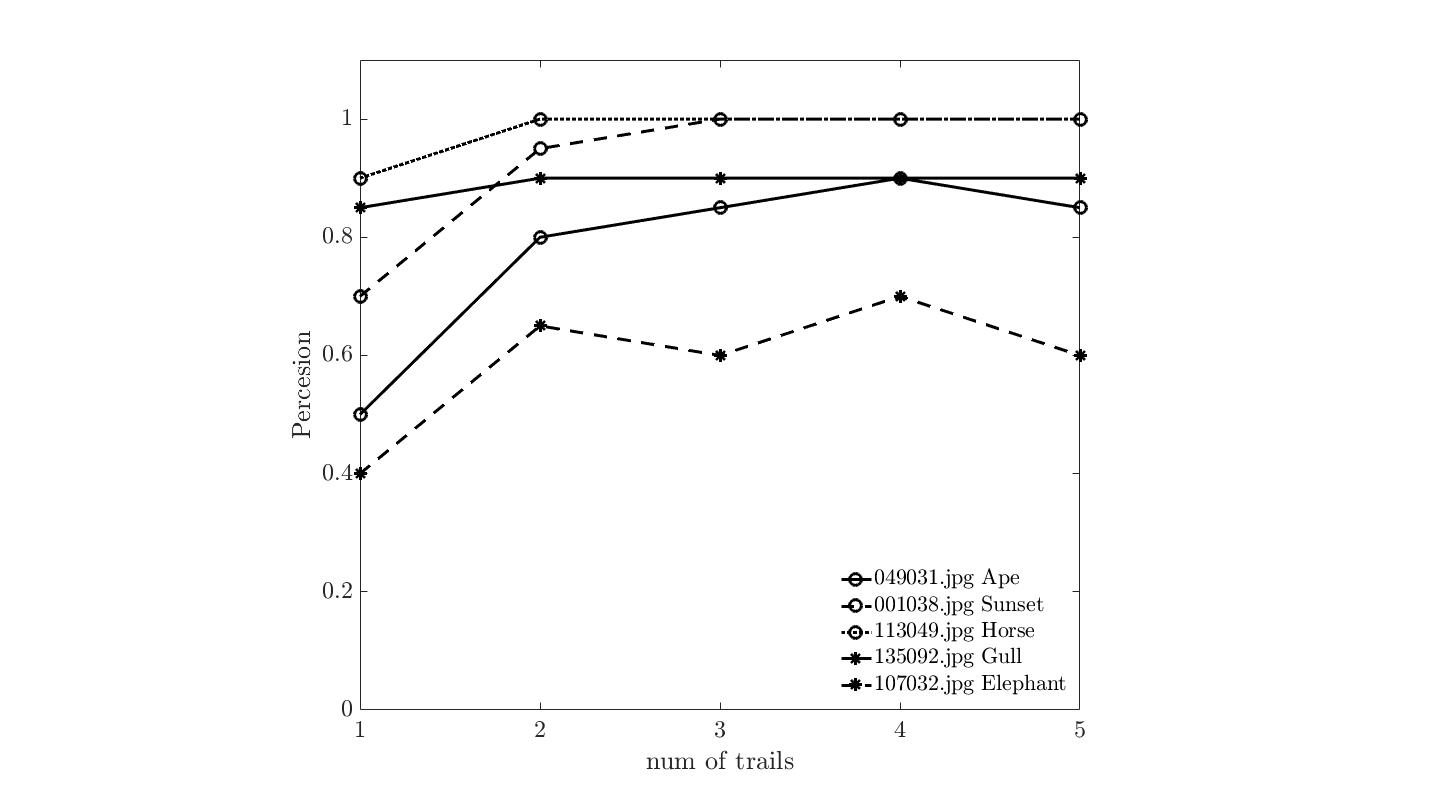
\includegraphics[width=\linewidth]{extra_credit}
			\caption{Percision with five rounds of query}
			\label{fig: 2}
		\end{figure}
		

        


\end{document}
